% -----------------------------------------------
% Template for SMC 2023
% based on SMC 2022 template
% -----------------------------------------------

\documentclass{article}
\usepackage{smc}
\usepackage{times}
\usepackage{ifpdf}
\usepackage[english]{babel}
\usepackage{cite}

%%%%%%%%%%%%%%%%%%%%%%%% Some useful packages %%%%%%%%%%%%%%%%%%%%%%%%%%%%%%%
%%%%%%%%%%%%%%%%%%%%%%%% See related documentation %%%%%%%%%%%%%%%%%%%%%%%%%%
%\usepackage{amsmath} % popular packages from Am. Math. Soc. Please use the 
%\usepackage{amssymb} % related math environments (split, subequation, cases,
%\usepackage{amsfonts}% multline, etc.)
%\usepackage{bm}      % Bold Math package, defines the command \bf{}
%\usepackage{paralist}% extended list environments
%%subfig.sty is the modern replacement for subfigure.sty. However, subfig.sty 
%%requires and automatically loads caption.sty which overrides class handling 
%%of captions. To prevent this problem, preload caption.sty with caption=false 
%\usepackage[caption=false]{caption}
%\usepackage[font=footnotesize]{subfig}


%user defined variables
\def\papertitle{Age Detection Image Processing: An approachhh}
\def\firstauthor{Luis Miguel Garcia Marin}
\def\secondauthor{Second author}
\def\thirdauthor{Third author}

% adds the automatic
% Saves a lot of output space in PDF... after conversion with the distiller
% Delete if you cannot get PS fonts working on your system.

% pdf-tex settings: detect automatically if run by latex or pdflatex
\newif\ifpdf
\ifx\pdfoutput\relax
\else
   \ifcase\pdfoutput
      \pdffalse
   \else
      \pdftrue
\fi

\ifpdf % compiling with pdflatex
  \usepackage[pdftex,
    pdfauthor={\firstauthor, \secondauthor, \thirdauthor},
    bookmarksnumbered, % use section numbers with bookmarks
    pdfstartview=XYZ % start with zoom=100% instead of full screen; 
                     % especially useful if working with a big screen :-)
   ]{hyperref}
  %\pdfcompresslevel=9

  \usepackage[pdftex]{graphicx}
  % declare the path(s) where your graphic files are and their extensions so 
  %you won't have to specify these with every instance of \includegraphics
  \graphicspath{{./figures/}}
  \DeclareGraphicsExtensions{.pdf,.jpeg,.png}

  \usepackage[figure,table]{hypcap}

\else % compiling with latex
  \usepackage[dvips,
    bookmarksnumbered, % use section numbers with bookmarks
    pdfstartview=XYZ % start with zoom=100% instead of full screen
  ]{hyperref}  % hyperrefs are active in the pdf file after conversion

  \usepackage[dvips]{epsfig,graphicx}
  % declare the path(s) where your graphic files are and their extensions so 
  %you won't have to specify these with every instance of \includegraphics
  \graphicspath{{./figures/}}
  \DeclareGraphicsExtensions{.eps}

  \usepackage[figure,table]{hypcap}
\fi

%setup the hyperref package - make the links black without a surrounding frame
\hypersetup{
    colorlinks,%
    citecolor=black,%
    filecolor=black,%
    linkcolor=black,%
    urlcolor=black
}


% Title.
% ------
\title{\papertitle}

% Authors
% Please note that submissions are NOT anonymous, therefore 
% authors' names have to be VISIBLE in your manuscript. 
%
% Single address
% To use with only one author or several with the same address
% ---------------
%\oneauthor
%   {\firstauthor} {Affiliation1 \\ %
%     {\tt \href{mailto:author1@smcnetwork.org}{author1@smcnetwork.org}}}

%Two addresses
%--------------
% \twoauthors
%   {\firstauthor} {Affiliation1 \\ %
%     {\tt \href{mailto:author1@smcnetwork.org}{author1@smcnetwork.org}}}
%   {\secondauthor} {Affiliation2 \\ %
%     {\tt \href{mailto:author2@smcnetwork.org}{author2@smcnetwork.org}}}

% Three addresses
% --------------
 \oneauthor
   {\firstauthor} {Fulda University of Applied Science \\ %
     {\tt \href{mailto:luis-miguel.garcia-marin@informatik.hs-fulda.de}{luis-miguel.garcia-marin@informatik.hs-fulda.de}}}


% ***************************************** the document starts here ***************
\begin{document}
%
\capstartfalse
\maketitle
\capstarttrue

\tableofcontents


\begin{abstract}
In this paper we introduce ourselves into the understanding of how we try to guess the age of a person just by looking at them and how this was tried to be implemented with different approaches of Machine Learning. We also see the results of my own approach with Convolutional Neural Networks (CNN), whose code it is provided in the references\cite{luis2021ageDetector}.
\end{abstract}


%\begin{figure}[hbt!]
%\centering
%\includegraphics[width=0.75\linewidth]{Lanzamiento de bolos.jpg}
%\caption{Bowling ball hitting the first bowl whit an angle of six degrees and the succession of strokes that will occur}
%\label{fig_sim}
%\end{figure}


\section{Introduction}\label{sec:introduction}

For sure you have asked before how old could be that person that you met the other day in the cafe or your favourite place and who took all your attention. We usually look at wrinkles in the skin, the texture and color of the hair or other facial or body features to try to guess a person's age. It could surprise us in how many features do our brain focus to try to guess this (even in their emotions\cite{monk2003adolescent}), and it was also studied in deep by many researchers\cite{aylward2005brain}.

\subsection{Starting to solve it}
Traditionally, detecting the age and gender of a person given an image of him or she has been an exciting task to solve along years. Initially, the problem was tried to be solved with traditional Machine Learning techniques\cite{wallinga2002detection} and with the principals that humans usually follows (like focusing in wrinkles in the skin, color of the hair...) as we mentioned before. But this approach did not get very successful results, since modelling all of this features was definitely not an easy task and they had to do many simplifications.

\subsection{Our approach}
I propose an approach with modern Deep Learning techniques, using the library TensorFlow\cite{tensorflow} in Python\cite{python} to build a model with enough successful results. The goal is not to build the best Neural Network for this purpose, but to give my own try and see the results.


\section{State of the Art}
\label{sec:state_of_the_art}

Nowadays we can see a lot of work related to the age detection, since the improvement of the Machine Learning techniques and how the Deep Learning has revolutionized it. But some ages before, were also related work to this field using traditional Machine Learning techniques, as we mentioned before\cite{wallinga2002detection}. Steven E. Campana, M. Christina Annand and James I. McMillan tried to determine the consistency with Graphical and Statistical Methods\cite{campana1995graphical}. But one of the first works that presented practical computations for visual age classification from facial images was in 1999 by Kwon, Young H and da Vitoria Lobo and Niels\cite{kwon1999age}.

Some decades after, everyone can make their own model for age detection with their own Personal Computer and Deep Learning tools. For example, Prerak Agarwal\cite{prerak2020} tried to solve this problem using traditional Machine Learning (using models like RandomForestClassifier or SVC) and Deep Learning techniques and compared the results, having a validation accuracy of 83.0\% with Convolutional Neural Networks while with SVC the best result was of 53.4\%. These results mean that the improvement in the use of CNN is clear.


\section{Methodology}\label{sec:methodology}

\subsection{Getting the data}
Before starting building the CNN model that we are going to train, we need the main ingredient in this recipe, which can not be other than the data. Some people try to make their own data of images and labels, taking a big amount of facial photos and assign to all of them a label, but this is a really tedious task. Therefore, I am going to use a dataset that I found in Kaggle.com\cite{nipun2020}, from Nipun Arora. This streamlines my workflow considerably.

This dataset provided by Nipun Arora includes 27305 facial images of 48x48 pixels from people aged between 1 and 93 years, and they are labeled on the basis of age, gender and ethnicity. This means that it can be used for many more purposes, but in our case this is more than enough. We can see the amount of images that we have classified by age, gender and ethnicity in the Figure \ref{fig:dataset}.

\begin{figure}[t]
\centering
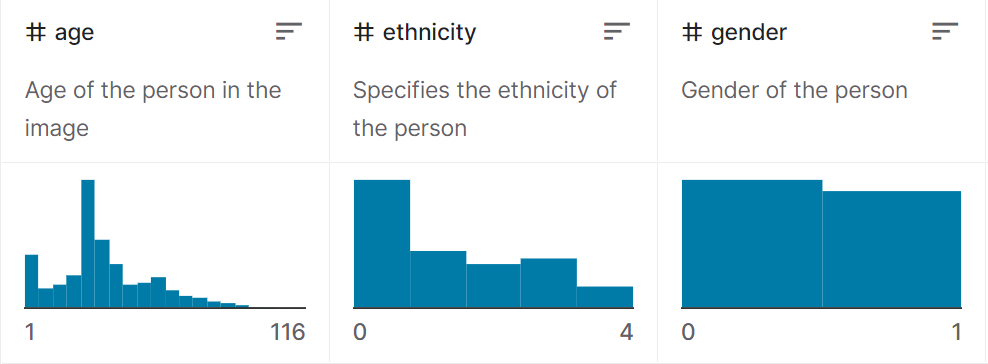
\includegraphics[width=1\columnwidth]{dataset-properties.png}
\caption{Amount of images of the dataset classified by age, gender and ethnicity.\label{fig:dataset}}
\end{figure}

\subsection{Technologies, tools and libraries}

As I mentioned before, for this approach I am going to use TensorFlow\cite{tensorflow}, a Google end-to-end machine learning platform, and Python\cite{python}, a programming language very commonly used for machine learning projects. But this is not enough, we need some more libraries: Numpy and Pandas for correctly loading, managing and operating dataframes (or tensors) of the dataset, Matplotlib for showing plots and graphics of our data, Keras to get the necessary layers to build our model, and Sklearn to use its "Train Test Split" function, in order to split our dataset into train and validation datasets.

\subsection{Converting the pixels of the data to a Numpy array}

Once we load the dataset of 27305 facial images of 48x48 pixels with their labels, in our case in .csv format, using Pandas and we explore the data, we see that the pixels are expressed as strings separated by spaces. To better handle this data, we are going to convert it into an array of numbers, with the help of a lambda function, which uses the functions x.split() (to separate the elements by each space) and np.array() (to build the array, with 32 precision float number type). The result of this is that we can see now that the pixels are a numerical array.

\subsection{Visualizing the data}

After this conversion, we are now able to preview some images of the dataset. I am going to show about 20 images, using the plot function of Matplotlib and accompanied by all the labels. However, in the next steps I will only take the 'age' label, since it is the only one that it is useful for this purpose. A visualization of this can be seen in the Figure \ref{fig:visualization}.

\begin{figure}[t]
\centering
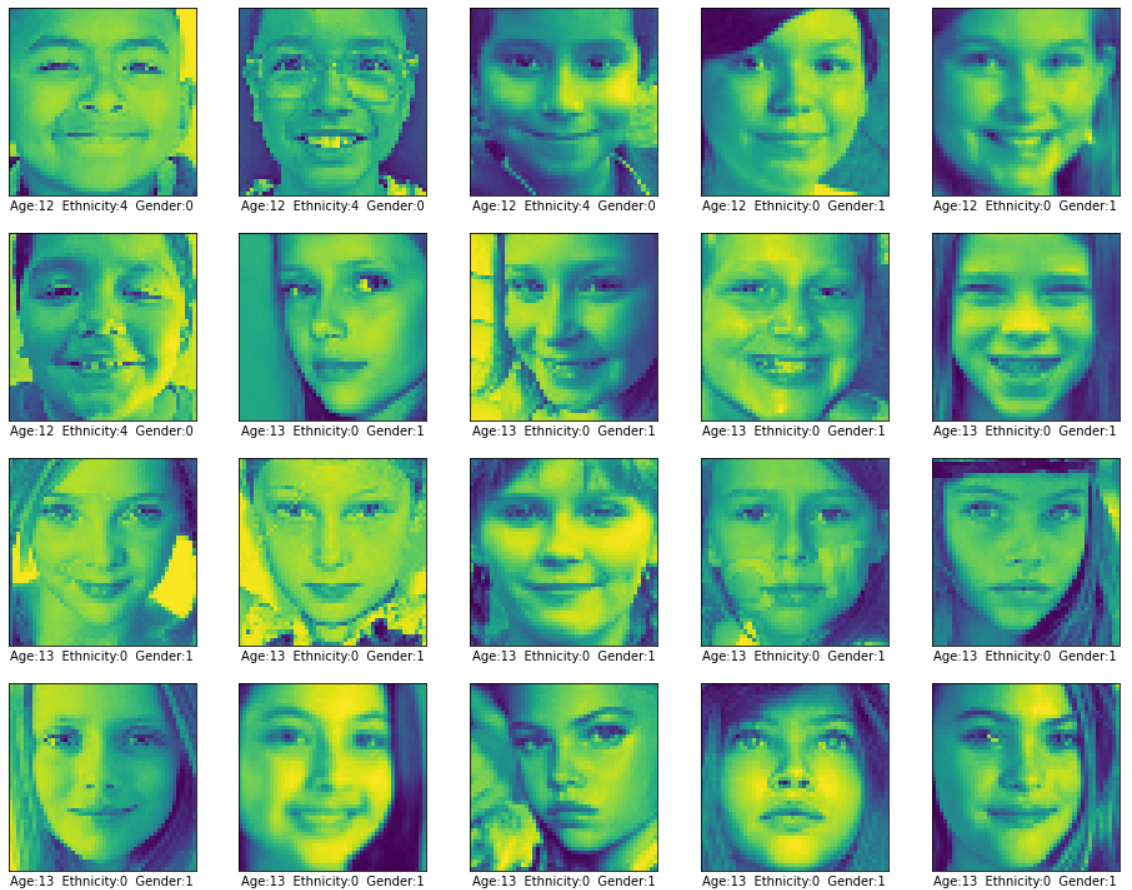
\includegraphics[width=1\columnwidth]{visualization_images.png}
\caption{Visualization of 20 images of the dataset with their labels.\label{fig:visualization}}
\end{figure}

\subsection{Processing the images}
Extracting the images:
We extract the pixels in a variable ("x"), converting them into a tuple to be able to correctly access the .shape attribute.
Normalizing the images:
We normalize the pixels so that the model can work better with floating values between 0 and 1. Knowing that the maximum value of a pixel is 255.
Converting pixels from 1D to 3D:
In order to have information about the nearby pixels and to be able to perform convolution, we now reshape the pixels to go from working with one dimension to three dimensions (width in pixels, height in pixels and number of color channels). In this way, the input of our neural network will also have these dimensions.

\subsection{Extracting the labels and spliting the datasets}
We get in another variable ("y") the age labels. Since there is no predefined total number of classes (the maximum age of a person does not have a strict limit), I am not going to categorize them.
After this, we are ready to split the datasets of images ("x") and labels ("y") into their train and test (also called validation) datasets respectively, and to do this, we use the "Train Test Split" function of the library Sklearn.

\subsection{Building the model}
We build the neural network model, in this case it is a modification of the one on the notebook 3 (Convolutional Neural Networks) of the Nvidia Deep Learning Introduction Course\cite{nvidiacourse}, used to detect the number in an image with the MNIST dataset. The input must be 3-dimensional as specified previously (48,48,1). However, we want the output to be a real number that indicates the predicted age of the person in the photo, so the output will be a single unit with Relu activation, since we do not have, as other times, a specific number of categories between which distribute the solution percentages.
You can see the summarizing of the model in the Figure \ref{fig:model}.

\begin{figure}[t]
\centering
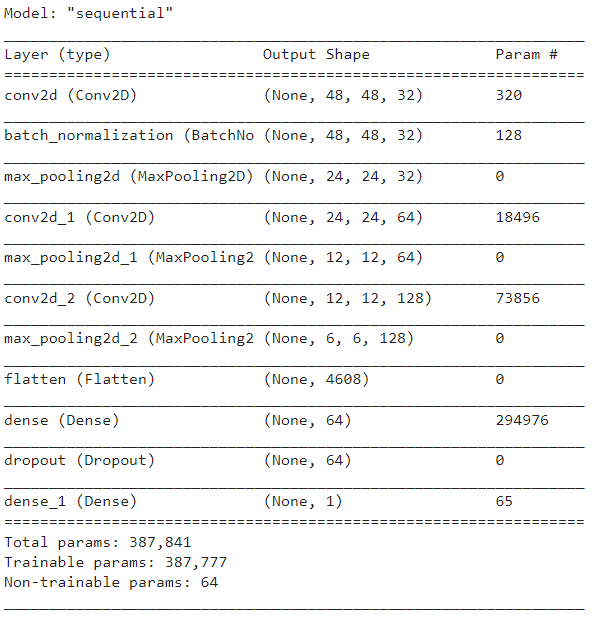
\includegraphics[width=1\columnwidth]{model-summary.png}
\caption{Summary of the Convolutional Neural Network model.\label{fig:model}}
\end{figure}

\subsection{Compiling and training the model}
In the compilation of the model we indicate to use 'adam' (method of the descent of the gradient stochastic) as an optimizer, the root mean square error as a loss function and the error mean absolute as metrics.
Then, we proceed to carry out the training of the model, with 20 epochs.


\section{Results}

As we can see from the Figure \ref{fig:training-model}, we end up obtaining loss value of 90.9845, but the most important value is the validation loss of 92.0247, which not differs so much from the training loss value, so we can confirm that there is no over-fitting in this train. We can also say that those values are not the best ones, but they are not bad ones either. This means that they are good enough to possibly have decent results, but the best way to see this is to test it with some examples.

\begin{figure}[t]
\centering
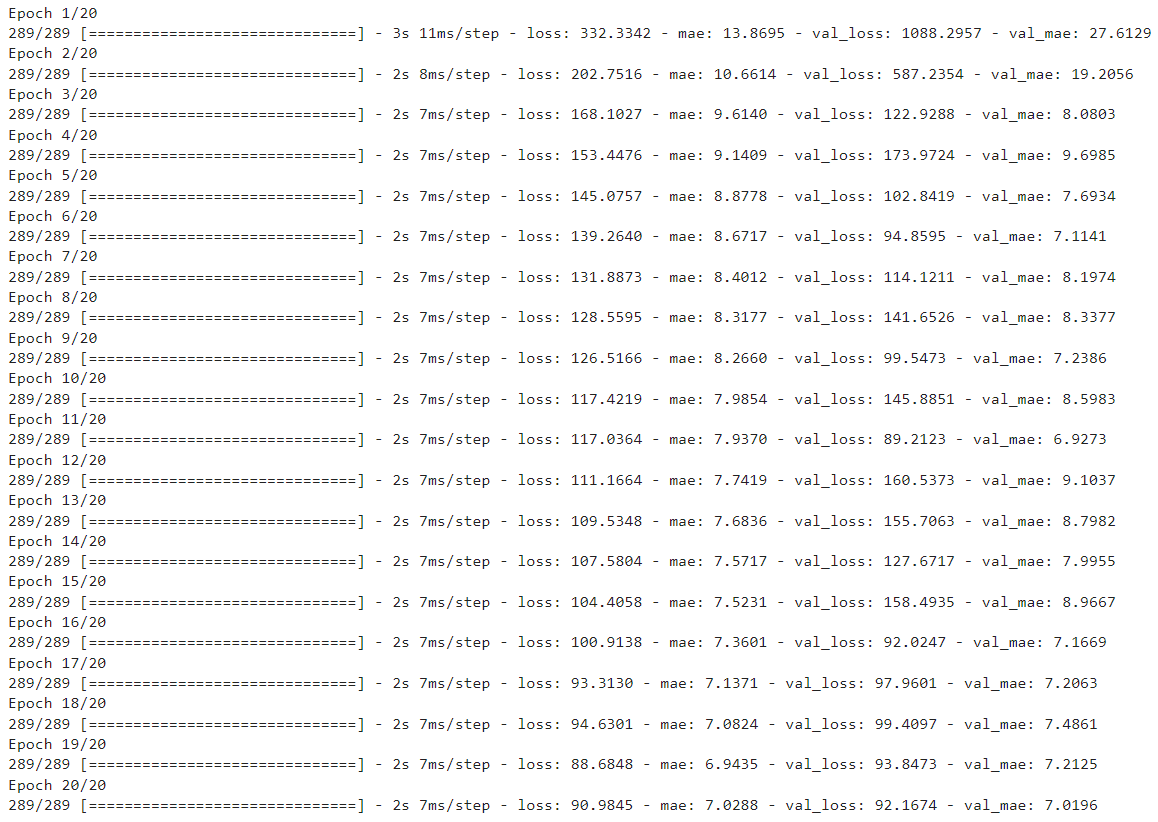
\includegraphics[width=1\columnwidth]{training-model.png}
\caption{Training results of the Convolutional Neural Network model.\label{fig:training-model}}
\end{figure}

Now, I create a make predictions function to make separate predictions and test the model. And then I finally create the age detector function, which makes use of the make predictions function and presents the result to us in a more legible way. I am going to use this function with 2 image examples: Princess Leonor's image (15 years old) and an old woman's image (90 years old). The results of these 2 examples can be seen in the Figure \ref{fig:testing-model}.

\begin{figure}[t]
\centering
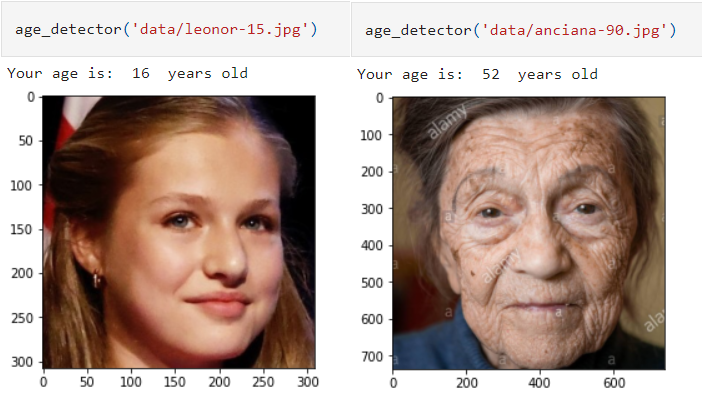
\includegraphics[width=1\columnwidth]{testing model.png}
\caption{Testing the Convolutional Neural Network model with 2 image examples.\label{fig:testing-model}}
\end{figure}

As we can see from this 2 experiments, the neural network predicts better the age of a younger person (the error is only of 1 year) than of an older person (the error in the second example is of 90 - 52 = 38 years), but what is this due to? 
This can be explained by looking at the amount of images of the used dataset classified by age (Figure \ref{fig:dataset}). We can see that there are more samples of persons with a young age than of older ages like 90 years old persons. Therefore, the neural network is not so trained for this situation. This could be solved by increasing the amount of the dataset by adding more images of elderly people.

\section{Discussion}

I introduced an approach to build a model for detecting the age of a person given their facial image and I found some ways in which this model could be improved and get better results. 

The future work could be increasing the variety of the dataset and making some changes in the layers of the model and test it in a heuristic way. In addition, I could try to expand the responsibilities of the model to predict also the gender and the ethnicity of a person based on their facial image.

But for the moment, this is good enough for experimentation and learning how to manage the Neural Network development. This is what it is behind the "Artificial Intelligence" which everyone is talking about, and it is not magic, it is just some adjustments and calculus in order to minimize the value of a loss function, as we have seen before.

Special thanks to Nvidia Deep Learning Institute Courses\cite{nvidiacourse}, from which I have learned many of the concepts and techniques presented here.

%%%%%%%%%%%%%%%%%%%%%%%%%%%%%%%%%%%%%%%%%%%%%%%%%%%%%%%%%%%%%%%%%%%%%%%%%%%%%
%bibliography here
\bibliography{smc2023bib}

\end{document}
